\documentclass[english,10pt]{beamer}

\mode<presentation>{
  \useinnertheme{rectangles}
  \usecolortheme[rgb={0.0,0.5,1.0}]{structure}
  \usecolortheme{orchid}
  \usecolortheme{whale}
  \useoutertheme{infolines}
  \setbeamercovered{transparent}
}

% packages
\usepackage{babel}
\usepackage[utf8]{inputenc}
\usepackage[T1]{fontenc}
\usepackage{lmodern}
\usepackage{graphicx}
\usepackage{wasysym}
\usepackage{relsize}
\usepackage{color}
\usepackage{verbatim}
\usepackage{listings}
\usepackage{algpseudocode}
\usepackage{tikz}
\usepackage{xspace}

\definecolor{version}{rgb}{1,0.5,0}

% Solarized colors
\definecolor{sbase03}{HTML}{002B36}
\definecolor{sbase02}{HTML}{073642}
\definecolor{sbase01}{HTML}{586E75}
\definecolor{sbase00}{HTML}{657B83}
\definecolor{sbase0}{HTML}{839496}
\definecolor{sbase1}{HTML}{93A1A1}
\definecolor{sbase2}{HTML}{EEE8D5}
\definecolor{sbase3}{HTML}{FDF6E3}
\definecolor{syellow}{HTML}{B58900}
\definecolor{sorange}{HTML}{CB4B16}
\definecolor{sred}{HTML}{DC322F}
\definecolor{smagenta}{HTML}{D33682}
\definecolor{sviolet}{HTML}{6C71C4}
\definecolor{sblue}{HTML}{268BD2}
\definecolor{scyan}{HTML}{2AA198}
\definecolor{sgreen}{HTML}{859900}

\lstloadlanguages{[11]C++}

\lstset{
  language=[11]C++,
  frame=lines,
  showstringspaces=false,
  xleftmargin=1ex,
  xrightmargin=1ex,
  % Light Solarized
  backgroundcolor=\color{sbase3},
  basicstyle=\ttfamily\color{sbase00},
  keywordstyle=\bfseries\color{scyan},
  commentstyle=\color{sbase1},
  stringstyle=\color{sblue},
  numberstyle=\color{sviolet},
  identifierstyle=\color{sbase00},
}

\title{Multi-Paradigm Programming}
\subtitle{Modern C++ programming}
\author{Julien BERNARD}
\institute[Univ. Franche-Comté]{Université de Franche-Comté, France}
\date{version 2025.1}

\AtBeginPart
{
  \frame{\partpage}
  \begin{frame}<beamer>
    \frametitle{Outline}
    \tableofcontents[subsubsectionstyle=hide]
  \end{frame}
}

\AtBeginSubsection[]
{
  \begin{frame}<beamer>
    \frametitle{Outline}
    \tableofcontents[currentsection,currentsubsection,subsubsectionstyle=show/show/hide/hide]
  \end{frame}
}

\AtBeginSubsubsection[]
{
  \begin{frame}<beamer>
    \frametitle{Outline}
    \tableofcontents[currentsection,currentsubsection,subsubsectionstyle=show/shaded/hide/hide]
  \end{frame}
}

\newcommand{\strong}[1]{\textbf{#1}}
\newcommand{\manualfootnote}{$^\dagger$}
\newcommand{\sourceinput}[1]{\vspace{-1ex}\smaller\lstinputlisting{#1}\larger\vspace{-1.2ex}}

\newcommand{\CCLang}{C\texttt{++}\xspace}
\newcommand{\CC}[1]{C\texttt{++}#1\xspace}
\newcommand{\Since}[1]{$^{\text{\bfseries\textcolor{version}{[C\texttt{++}#1]}}}$}

\begin{document}

\begin{frame}
  \titlepage
\end{frame}

\part{Introduction}

\section{Introduction}

\subsection{About this course}

\begin{frame}{Hello World}{}
  \begin{center}
    \sourceinput{snippets/hello.cc}

    \bigskip

    \begin{quote}
      "There are only two kinds of languages: the ones people complain about and the ones nobody uses."
      \begin{flushright}
        \upshape Bjarne Stroustrup, creator of \CCLang
      \end{flushright}
    \end{quote}
  \end{center}
\end{frame}

\begin{frame}{Objective and scope}{}
  \begin{block}{Objective}
    Learn how to use different paradigms in a single application with modern \CCLang

    \begin{itemize}
    \item
      procedural programming
    \item
      object-oriented programming
    \item
      functional programming
    \item
      generic programming
    \end{itemize}
  \end{block}

  \begin{block}{Scope}
    \begin{itemize}
    \item
      \strong{Not} the basics of programming and/or the basics of \CCLang
    \item
      The elements to understand how \CCLang works
    \item
      The idioms and good practices of \CCLang
    \end{itemize}
  \end{block}
\end{frame}

\begin{frame}{Organisation}{}
  \begin{block}{Hours}
    \begin{itemize}
    \item
      Lecture: 5 $\times$ 1h30
    \item
      Test: 1 $\times$ 1h30
    \item
      Laboratory: 6 $\times$ 3h00
    \end{itemize}
  \end{block}

  \begin{block}{Evaluation}
    \begin{itemize}
    \item
      Multiple choice test (50\%)
    \item
      Laboratory project in \CCLang (50\%)
    \end{itemize}
  \end{block}
\end{frame}

\begin{frame}{Resources}{}
  \begin{block}{Online}
    \begin{itemize}
    \item
      \CCLang Reference: \url{http://en.cppreference.com/w/cpp}
    \item
      \CCLang FAQ: \url{http://isocpp.org/faq}
    \item
      \CCLang Core Guidelines: \url{https://github.com/isocpp/CppCoreGuidelines/}
    \end{itemize}
  \end{block}

  \begin{block}{Books}
    \begin{thebibliography}{}
    \bibitem{Stroustrup}
      Bjarne Stroustrup.
      \newblock {\em The \CCLang Programming Language}.
      \newblock 4th edition, 2013, Addison--Wesley
    \end{thebibliography}
  \end{block}
\end{frame}

\subsection{\CCLang Origins}

% Source: "Evolving a language in and for the real world: 1991-2006", Bjarne Stroustrup

\begin{frame}{\CCLang History (1/3)}{Early \CCLang}
  \begin{block}{Early \CCLang (1979--1998)}
    \begin{itemize}
    \item
      1979: "C with Classes", Bjarne Stroustrup, AT\&T Bell Labs
    \item
      1983: "C with Classes" $\leadsto$ \CCLang; CFront 1.0
    \item
      1985: \emph{The \CCLang Programming Language}, 1st edition, Bjarne Stroustrup
    \item
      1989: \emph{The Annotated \CCLang Reference Manual}, Bjarne Stroustrup; CFront 2.0
    \item
      1991: First ISO/IEC JTC1/SC22/WG21 meeting; CFront 3.0
    \item
      1992: \emph{Effective \CCLang}, 1st edition, Scott Meyers
    \item
      1993: Standard Template Library, Alexander Stepanov, HP Labs
    \item
      1994: \emph{The Design and Evolution of \CCLang}, Bjarne Stroustrup
    \item
      1998: \emph{Effective \CCLang}, 2nd edition, Scott Meyers
    \end{itemize}
  \end{block}
\end{frame}

\begin{frame}{\CCLang History (2/3)}{Standard \CCLang}
  \begin{block}{Standard \CCLang (1998--2011)}
    \begin{itemize}
    \item
      1998: ISO standardization, \CC{98}
    \item
      2001: \emph{Modern \CCLang Design}, Andrei Alexandrescu
    \item
      2003: \CC{03}, minor revision
    \item
      2005: \emph{Effective \CCLang}, 3rd edition, Scott Meyers
    \item
      2006: Performance Technical Report
    \item
      2007: Library Technical Report 1 (TR1)
    \end{itemize}
  \end{block}
\end{frame}

\begin{frame}{\CCLang History (3/3)}{Modern \CCLang}
  \begin{block}{Modern \CCLang (2011--)}
    \begin{itemize}
    \item
      2011: \CC{11}, major revision
      \begin{itemize}
      \item[$\to$]
        "Surprisingly, \CC{11} feels like a new language"
      \end{itemize}
    \item
      2012: Standard \CCLang Foundation
    \item
      2014: \CC{14}, minor revision; \emph{Effective Modern \CCLang}, Scott Meyers
    \item
      2015: \CCLang Core Guidelines, Guidelines Support Library
    \item
      2017: \CC{17}, major revision
    \item
      2020: \CC{20}, next major revision of the standard
    \end{itemize}
  \end{block}
\end{frame}

\begin{frame}{Design Rules (1/4)}{General rules}
  \begin{block}{General rules}
    \begin{enumerate}
    \item
      \CCLang's evolution must be driven by real problems.
    \item
      Don't get involved in a sterile quest for perfection.
    \item
      \CCLang must be useful \emph{now}.
    \item
      Every feature must have a reasonably obvious implementation.
    \item
      Always provide a transition path.
    \item
      \CCLang is a language, not a complete system.
    \item
      Provide comprehensive support for each supported style.
    \item
      Don't try to force people to use a specific programming style.
    \end{enumerate}
  \end{block}
\end{frame}

\begin{frame}{Design Rules (2/4)}{Design support rules}
  \begin{block}{Design support rules}
    \begin{enumerate}
    \item
      Support sound design notions.
    \item
      Provide facilities for program organization.
    \item
      Say what you mean.
    \item
      All features must be affordable.
    \item
      It is more important to allow a useful feature than to prevent every misuse.
    \item
      Support composition of software from separately developed parts.
    \end{enumerate}
  \end{block}
\end{frame}

\begin{frame}{Design Rules (3/4)}{Language-technical rules}
  \begin{block}{Language-technical rules}
    \begin{enumerate}
    \item
      No implicit violations of the static type system.
    \item
      Provide as good support for user-defined types as for built-in types.
    \item
      Locality is good.
    \item
      Avoid order dependencies.
    \item
      If in doubt, pick the variant of a feature that is easiest to teach.
    \item
      Syntax matters (often in perverse ways).
    \item
      Preprocessor usage should be eliminated.
    \end{enumerate}
  \end{block}
\end{frame}

\begin{frame}{Design Rules (4/4)}{Low-level programming support rules}
  \begin{block}{Low-level programming support rules}
    \begin{enumerate}
    \item
      Use traditional (dumb) linkers.
    \item
      No gratuitous incompatibilities with C.
    \item
      Leave no room for a lower-level language below C++ (except assembler).
    \item
      What you don’t use, you don’t pay for (zero-overhead rule).
    \item
      If in doubt, provide means for manual control.
    \end{enumerate}
  \end{block}
\end{frame}

\subsection{\CCLang Paradigms}

\begin{frame}{Programming paradigm}{}
  \begin{definition}[Programming paradigm]
    A \strong{programming paradigm} is a way to think about the execution and/or the organization of a program. A programming paradigm enables some constructs in a language and forbids other constructs.
  \end{definition}

  \begin{block}{Remarks}
    \begin{itemize}
    \item
      There are dozens of programming paradigms.
    \item
      Most languages can be classified into multiple paradigms (like \CCLang).
    \end{itemize}
  \end{block}

  \begin{example}[Imperative programming]
    \strong{Imperative programming} is a paradigm that uses a sequence of statements to change the program's state.
  \end{example}
\end{frame}

\begin{frame}{Procedural programming}{}
  \begin{definition}[Procedural programming]
    \strong{Procedural programming} is an imperative programming paradigm based on the concept of \emph{procedure call}.
  \end{definition}
  \begin{block}{Procedural programming in \CCLang}
    \CCLang is a procedural programming language.
    \begin{itemize}
    \item
      Modularity through function parameters and return values
    \item
      Function call from any other function
    \item[$\to$]
      C style
    \end{itemize}
  \end{block}
\end{frame}

\begin{frame}{Object-oriented programming}{}
  \begin{definition}[Object-oriented programming]
    \strong{Object-oriented programming} is an imperative programming paradigm based based on the concepts of \emph{objects} (data) and \emph{methods} (code).
  \end{definition}
  \begin{block}{Object-oriented programming in \CCLang}
    \CCLang is an object-oriented programming language.
    \begin{itemize}
    \item
      Classes (\lstinline!class!)
      \begin{itemize}
      \item[$\to$]
        Class-based object-oriented programming ($\neq$ Prototype-based)
      \end{itemize}
    \item
      Composition and (multiple) inheritance
    \item
      Polymorphism (\lstinline!virtual! methods, \lstinline!dynamic_cast!)
    \end{itemize}
  \end{block}
\end{frame}

\begin{frame}{Functional programming}{}
  \begin{definition}[Functional programming]
    \strong{Functional programming} is a programming paradigm based on the concept of \emph{mathematical functions} and forbids side effects (no assignment).
  \end{definition}
  \begin{block}{Functional programming in \CCLang}
    \CCLang is \strong{not} a functional programming language\ldots
    \begin{itemize}
    \item
      No currying
    \end{itemize}
    \ldots but has elements of a functional programming language.
    \begin{itemize}
    \item
      Recursion
    \item
      Functors and lambda functions\Since{11} (closures)
    \item
      \lstinline!std::function!\Since{11}
    \item
      Partial evaluation (\lstinline!std::bind!)
    \end{itemize}
  \end{block}
\end{frame}

\begin{frame}{Generic programming}{}
  \begin{definition}[Generic programming]
    \strong{Generic programming} is a programming paradigm where types and algorithms are defined with abstract type parameters.
  \end{definition}
  \begin{block}{Generic programming in \CCLang}
    \CCLang is a generic programming language.
    \begin{itemize}
    \item
      Templates
    \item
      Standard Template Library (STL): containers, iterators, algorithms
    \item
      Concepts\Since{20}
    \end{itemize}
  \end{block}
\end{frame}

\begin{frame}{Using multiple paradigms}{}
  \begin{example}
    \sourceinput{snippets/multi_paradigm.cc}

    \begin{itemize}
    \item
      Procedural: \lstinline!drawAll()!
    \item
      Object-oriented: \lstinline!shape->draw()!
    \item
      Functional: \lstinline![](const Shape *shape) \{ \}!
    \item
      Generic: \lstinline!std::vector<Shape*>! and \lstinline!std::for_each!
    \end{itemize}
  \end{example}
\end{frame}


\section{Expressions, declarations and statements in \CCLang}

\subsection{Overview}

\begin{frame}{\CCLang program}{}
  \begin{definition}[\CCLang program]
    A \strong{\CCLang program} is a sequence of text files (typically header and source files) that contain declarations. They undergo translation to become an executable program, which is executed when the C++ implementation calls its main function.
  \end{definition}
\end{frame}

\begin{frame}{Entities}{}
  \begin{block}{Entities}
    The \strong{entities} of a C++ program are:
    \begin{itemize}
    \item
      values
    \item
      objects
    \item
      references
    \item
      structured bindings\Since{17}
    \item
      functions
    \item
      enumerators
    \item
      types
    \item
      class members
    \item
      templates
    \item
      template specializations
    \item
      namespaces
    \item
      parameter packs.
    \end{itemize}
  \end{block}
\end{frame}

\begin{frame}{Objects}{}
  \begin{definition}[Object]
    An \strong{object} is a \emph{region of storage} with the following properties:
    \begin{itemize}
    \item
      a size (that can be determined with \lstinline!sizeof!)
    \item
      an alignment requirement (that can be determined with \lstinline!alignof!)
    \item
      a storage duration (automatic, static, dynamic, thread-local)
    \item
      a lifetime
    \item
      a type
    \item
      a value (which may be indeterminate)
    \item
      optionally, a name
    \end{itemize}
  \end{definition}
\end{frame}


\subsection{Value categories}

\begin{frame}{Expressions}{}
  \begin{block}{Expressions}
    Expressions are characterized by two properties:
    \begin{itemize}
    \item
      a \emph{type}
    \item
      a \emph{value category}
    \end{itemize}
  \end{block}

  \begin{block}{Value categories before \CC{11}}
    \begin{itemize}
    \item
      An \strong{lvalue expression} identifies an object ("locator value")
      \begin{itemize}
      \item[$\approx$]
        what is on the left-hand side  of an assignment
      \end{itemize}
    \item
      A \strong{rvalue expression} is an expression that is not an lvalue expression
      \begin{itemize}
      \item[$\approx$]
        what is on the right-hand side of an assignment
      \end{itemize}
    \end{itemize}
  \end{block}
\end{frame}

\begin{frame}{Value categories}{Overview}
  \begin{block}{Value categories}
    \begin{itemize}
    \item
      Primary categories: lvalue, prvalue, xvalue
    \item
      Mixed categories: glvalue, rvalue
    \end{itemize}
  \end{block}

  \begin{center}
    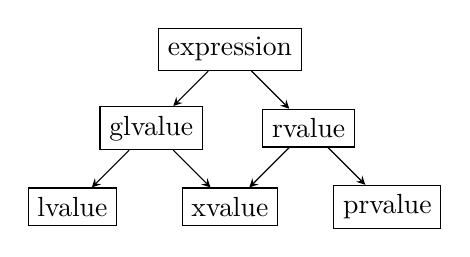
\begin{tikzpicture}
      \node[draw] (E) at ( 0, 0) { expression } ;
      \node[draw] (G) at (-1,-1) { glvalue } ;
      \node[draw] (R) at ( 1,-1) { rvalue } ;
      \node[draw] (L) at (-2,-2) { lvalue } ;
      \node[draw] (X) at ( 0,-2) { xvalue } ;
      \node[draw] (P) at ( 2,-2) { prvalue } ;

      \draw[->,>=stealth] (E) -- (G) ;
      \draw[->,>=stealth] (E) -- (R) ;
      \draw[->,>=stealth] (G) -- (L) ;
      \draw[->,>=stealth] (G) -- (X) ;
      \draw[->,>=stealth] (R) -- (X) ;
      \draw[->,>=stealth] (R) -- (P) ;
    \end{tikzpicture}
  \end{center}
\end{frame}

% http://www.open-std.org/jtc1/sc22/wg21/docs/papers/2015/p0135r0.html
\begin{frame}{Value categories}{Definition (\CC{17})}
  \begin{definitions}[Value categories]
    \begin{itemize}
    \item
      A \strong{glvalue} ("generalized" lvalue) is an expression whose evaluation determines the identity of an object, bit-field, or function
      \begin{itemize}
      \item[$\to$]
        \emph{glvalues produce locations}
      \end{itemize}
    \item
      A \strong{prvalue} ("pure" rvalue) is an expression whose evaluation either:
      \begin{itemize}
      \item
        computes the value of the operand of an operator (has no result object), or
      \item
        initializes an object or a bit-field (has a result object)
      \item[$\to$]
        \emph{prvalues perform initialization}
      \end{itemize}
    \item
      An \strong{xvalue} (eXpiring value) is a glvalue that denotes an object or bit-field whose resources can be reused (usually near the end of its lifetime)
    \item
      An \strong{lvalue} is a glvalue that is not an xvalue
    \item
      An \strong{rvalue} is a prvalue or an xvalue.
    \end{itemize}
  \end{definitions}
\end{frame}

\begin{frame}{Properties of glvalues and rvalues}{}
  \begin{block}{Properties of a glvalue expression (lvalue or xvalue)}
    \begin{itemize}
    \item
      May be converted to a prvalue
    \item
      May be polymorphic (dynamic type $\neq$ static type)
    \item
      Can have incomplete type
    \end{itemize}
  \end{block}

  \begin{block}{Properties of a rvalue expression (prvalue or xvalue)}
    \begin{itemize}
    \item
      Has no address
    \item
      Can not be used as the left-hand of the built-in assignment operator
    \item
      May be used to initialize a const lvalue reference or an rvalue reference
      \begin{itemize}
      \item[$\to$]
        In that case, the lifetime of the object identified by the rvalue is extended until the scope of the reference ends
      \end{itemize}
    \end{itemize}
  \end{block}
\end{frame}

\begin{frame}{Properties of lvalues and prvalues}{}
  \begin{block}{Properties of an lvalue expression}
    \begin{itemize}
    \item
      Has an address
    \item
      If modifiable, may be used as the left-hand of the built-in assignment operator
    \item
      May be used to initialize an lvalue reference
    \end{itemize}
  \end{block}

  \begin{block}{Properties of an prvalue expression}
    \begin{itemize}
    \item
      Can not be polymorphic
    \item
      If non-class and non-array, can not be cv-qualified
    \item
      Can not have incomplete type
    \item
      Can not have abstract class type
    \end{itemize}
  \end{block}
\end{frame}

\begin{frame}{Examples of lvalues}{}
  \begin{examples}[lvalue expressions]
    \begin{itemize}
    \item
      Name of a variable, function, data member (\lstinline!std::cin!)
    \item
      Function call or overloaded operator expression whose return type is lvalue reference (\lstinline!std::getline(std::cin, str)!, \lstinline!std::cout << 1!, \lstinline!++it!)
    \item
      Assignment and compound assignment expressions (\lstinline!a = b!, \lstinline!a += b!)
    \item
      Builtin pre-increment and pre-decrement expressions (\lstinline!++i!)
    \item
      Builtin indirection expression (\lstinline!*p!)
    \item
      Builtin subscript operator\manualfootnote (\lstinline!a[n]!)
    \item
      String literal (\lstinline!"Hello"!)
    \item
      Member of object expressions\manualfootnote (\lstinline!a.m!)
    \item
      Built-in member of pointer expression\manualfootnote (\lstinline!a->m!)
    \end{itemize}

    \raggedleft
    \footnotesize
    \manualfootnote with exceptions
  \end{examples}
\end{frame}

\begin{frame}{Examples of prvalues}{}
  \begin{examples}[prvalue expressions]
    \begin{itemize}
    \item
      Literal\manualfootnote (\lstinline!42!, \lstinline!true!, \lstinline!nullptr!)
    \item
      Function call or an overloaded operator expression whose return type is non-reference (\lstinline!str.substr(1, 2)!, \lstinline!it++!)
    \item
      Builtin post-increment and post-decrement expressions (\lstinline!i++!)
    \item
      Builtin arithmetic expressions (\lstinline!a + b!, \lstinline!a / b!, \lstinline!a & b!, \lstinline!a << b!, \lstinline!-a!)
    \item
      Builtin logical expressions (\lstinline!a && b!, \lstinline!a || b!, \lstinline|!a|)
    \item
      Builtin comparison expressions (\lstinline!a < b!, \lstinline!a == b!)
    \item
      Builtin address-of expression (\lstinline!&a!)
    \item
      The \lstinline!this! pointer
    \item
      Enumerator
    \item
      Lambda expression (\lstinline![](int x) \{ return x * x; \}!)
    \end{itemize}

    \raggedleft
    \footnotesize
    \manualfootnote with exceptions
  \end{examples}
\end{frame}

\begin{frame}{Examples of xvalues}{}
  \begin{examples}[xvalue expressions]
    \begin{itemize}
    \item
      Function call or an overloaded operator expression, whose return type is rvalue reference to object (\lstinline!std::move(x)!)
    \item
      Expression that designates a temporary object
    \end{itemize}
  \end{examples}
\end{frame}

\begin{frame}{Determination of the value category}{}
  \begin{block}{lvalue or rvalue?}
    \begin{enumerate}
    \item
      Determine if the expression is a glvalue or a prvalue
      \begin{itemize}
      \item
        glvalues produce locations
      \item
        prvalues perform initialization
      \end{itemize}
    \item
      If glvalue, determine if the expression is a temporary object or not
      \begin{itemize}
      \item
        Temporary objects are xvalues
      \item
        Non-temporary objects are lvalues
      \end{itemize}
    \item[$\to$]
      prvalues and xvalues are rvalues, everything else is an lvalue
    \end{enumerate}
  \end{block}
\end{frame}

% TODO: example

\subsection{Memory allocation}

\begin{frame}{\texttt{new} expression}{}
  \begin{block}{\texttt{new} expression}
    A \lstinline!new! expression allocates and initializes objects with dynamic storage duration.

    {
      \hfill\lstinline[mathescape]!new $\;type\;$! or \lstinline[mathescape]!new $\;type\;$ $\;initializer\;$!\hfill
    }
    \begin{itemize}
    \item
      Attempts to allocate storage and then attempts to construct and initialize either a single unnamed object, or an unnamed array of objects in the allocated storage
    \item
      Returns a prvalue pointer to the constructed object or, if an array of objects was constructed, a pointer to the initial element of the array
    \end{itemize}
  \end{block}

  \begin{example}[\texttt{new} expression]
    \sourceinput{snippets/new.cc}
  \end{example}
\end{frame}

\begin{frame}{Placement \texttt{new} expression}{}
  \begin{block}{Placement \texttt{new} expression}
    A placement \lstinline!new! expression is used to construct objects in an already allocated storage

    {
      \hfill\lstinline[mathescape]!new ($\;placement\;$) $\;type\;$! or \lstinline[mathescape]!new ($\;placement\;$) $\;type\;$ $\;initializer\;$!\hfill
    }
  \end{block}

  \begin{example}[Placement \texttt{new} expression]
    \sourceinput{snippets/placement_new.cc}
  \end{example}
\end{frame}

\begin{frame}{\texttt{delete} expression}{}
  \begin{block}{\texttt{delete} expression}
    A \lstinline!delete! expression destroys the object(s) previously allocated by a \lstinline!new! expression and releases the obtained memory area.

    {
      \hfill\lstinline[mathescape]!delete $\;expr\;$!\hfill
    }
    \begin{itemize}
    \item
      Destroys one non-array object created by a new-expression
    \item
      \lstinline[mathescape]!$expr$! can be \lstinline!nullptr!
    \end{itemize}
    {
      \hfill\lstinline[mathescape]!delete [] $\;expr\;$!\hfill
    }
    \begin{itemize}
    \item
      Destroys an array created by a new[]-expression
    \item
      \lstinline[mathescape]!$expr$! can be \lstinline!nullptr!
    \end{itemize}
  \end{block}

  \begin{block}{Remark}
    Never mix non-array \lstinline!new!/\lstinline!delete! and array \lstinline!new[]!/\lstinline!delete[]!!
  \end{block}
\end{frame}

\begin{frame}{Good practice for memory allocation}{}
  \begin{block}{Good practice for memory allocation}
    \begin{center}
      \Large
      \bfseries
      Never use \lstinline!new! and \lstinline!delete!!
    \end{center}

    Use smart pointers according to ownership semantics:
    \begin{itemize}
    \item
      Unique object $\to$ \lstinline!std::unique_ptr<T>! and \lstinline!std::make_unique!\Since{14}
    \item
      Shared object $\to$ \lstinline!std::shared_ptr<T>! and \lstinline!std::make_shared!
    \end{itemize}
  \end{block}

  \begin{example}[Smart pointers]
    \sourceinput{snippets/smart_pointers.cc}
  \end{example}
\end{frame}


\subsection{Scoped enumerations}

\begin{frame}{Scoped enumeration}{}
  \begin{block}{Scoped enumeration}
    {
      \hfill\lstinline[mathescape]!enum class $\;name\;$ \{ $\;enumerators\;$ \}!\hfill
    }

    \begin{itemize}
    \item
      The underlying type is \lstinline!int!
    \item
      The enumerators are contained in the scope of the enumeration
    \item
      The enumerators can be accessed using scope resolution operator \lstinline!::!
    \item
      \lstinline!static_cast! is required to obtain the numeric value of the enumerator
    \end{itemize}

    {
      \hfill\lstinline[mathescape]!enum class $\;name\;$ : $\;type\;$ \{ $\;enumerators\;$ \}!\hfill
    }

    \begin{itemize}
    \item
      The underlying type is \lstinline[mathescape]!$type$!
    \item
      \lstinline[mathescape]!$type$! is an integral type
    \end{itemize}
  \end{block}

  \begin{block}{Remark}
    Always use scoped enumerations!
  \end{block}
\end{frame}

\begin{frame}{Scoped enumeration}{}
  \begin{example}[Scoped enumeration]
    \sourceinput{snippets/scoped_enum.cc}
  \end{example}
\end{frame}

\subsection{References}

\begin{frame}{References}{}
  \begin{definitions}[References]
    A \strong{reference} of type~\lstinline!T! is an alias to an already existing object or function of type~\lstinline!T!. There are two types of references.
    \begin{itemize}
    \item
      A \strong{lvalue reference}, noted \lstinline!T&!, can be used to:
      \begin{itemize}
      \item
        Alias an lvalue
      \item
        Implement pass-by-reference semantics in function calls
      \item
        Be the return type of a function, the function call is an lvalue expression
      \end{itemize}
    \item
      A \strong{rvalue references}, noted \lstinline!T&&!, can be used to:
      \begin{itemize}
      \item
        Extend the lifetime of a temporary object
      \item
        Create overloads for rvalue expressions
      \end{itemize}
    \end{itemize}
  \end{definitions}
\end{frame}

\begin{frame}{Limits of references}{}
  \begin{block}{Limits of references}
    \begin{itemize}
    \item
      There are no references to void
    \item
      A reference is required to be initialized to refer to a valid object or function
      \begin{itemize}
      \item[$\to$]
        A null reference can not exist
      \end{itemize}
    \item
      References are not objects (they do not necessarily require storage)
      \begin{itemize}
      \item[$\to$]
        There are no references to references
      \item[$\to$]
        There are no arrays of references
      \item[$\to$]
        There are no pointers to references
      \end{itemize}
    \end{itemize}
  \end{block}
\end{frame}

\begin{frame}{Reference initialization}{}
  \begin{block}{Reference initialization}
    References are initialized in the following situations:
    \begin{itemize}
    \item
      Variable declarations:
      \begin{itemize}
      \item
        Declaration of a named lvalue reference variable with an initializer
      \item
        Declaration of a named rvalue reference variable with an initializer
      \end{itemize}
    \item
      Functions (see part~2): % TODO: ~\ref{part:proc}):
      \begin{itemize}
      \item
        Function call expression, when the function parameter has reference type
      \item
        Return statement, when the function returns a reference type
      \end{itemize}
    \item
      Objects (see part~3): % TODO: \ref{part:oop}):
      \begin{itemize}
      \item
         Initialization of a non-static data member of reference type using a member initializer
      \end{itemize}
    \end{itemize}
  \end{block}
\end{frame}

\begin{frame}{References}{}
  \begin{examples}[References]
    \small
    \sourceinput{snippets/references.cc}
  \end{examples}
\end{frame}

\begin{frame}{\texttt{std::move}}{}
  \begin{block}{\texttt{std::move}}
    \lstinline!std::move! is used to \emph{indicate} that an object may be "moved from", i.e. allowing the efficient transfer of resources from an object to another object.

    In particular, \lstinline!std::move! produces an xvalue expression that identifies its argument.

    \begin{itemize}
    \item
      A \lstinline!std::move! is equivalent to a \lstinline!static_cast! to an rvalue reference type
    \item
      If a function accepts rvalue reference parameters, \lstinline!std::move! can be used to produce an xvalue
    \item
      Generally, a moved-from object is in a valid but unspecified state
    \end{itemize}
  \end{block}
\end{frame}

\begin{frame}{\texttt{std::move}}{}
  \begin{example}[\texttt{std::move}]
    \sourceinput{snippets/move.cc}
  \end{example}
\end{frame}


\subsection{Namespaces}

\begin{frame}{Namespace}{}
  \begin{definition}[Namespace]
  A \strong{namespace} is a named declarative region. The name of the namespace can be used to access the entities declared in that namespace.
  \end{definition}

  \begin{block}{Remarks}
    \begin{itemize}
    \item
      Multiple namespace blocks with the same name are allowed.
    \item
      The standard library lives in the \lstinline!std! namespace.
%     \item
%       Names not in a namespace are in the global namespace
    \end{itemize}
  \end{block}

  \begin{example}[Namespace]
    \sourceinput{snippets/namespace.cc}
  \end{example}
\end{frame}

\begin{frame}{Inline namespace}{}
  \begin{definition}[Inline namespace]
    An \strong{inline namespace} is a namespace whose members are treated as if they were members of the enclosing namespace.
  \end{definition}

  \begin{example}[Inline namespace]
    \sourceinput{snippets/namespace_inline.cc}
  \end{example}
\end{frame}

\begin{frame}{Inline namespace and versioning}{}
  \begin{block}{Versioning}
    Inline namespaces are useful for library versioning.
    \begin{enumerate}
    \item
      Put your declarations in an inline namespace \lstinline!v1!
    \item
      In case of ABI breakage, put the old declaration in a non-inline namespace \lstinline!v1! and the new declaration in an inline namespace \lstinline!v2! (and so on)
      \begin{itemize}
      \item
        The old declaration is still accessible for old users (no need to recompile)
      \item
        The new declaration is the default for new users
      \end{itemize}
    \end{enumerate}
  \end{block}
  \begin{example}[Inline namespace and versioning]
    \sourceinput{snippets/namespace_versioning.cc}
  \end{example}
\end{frame}

\begin{frame}{Unnamed namespace}{}
  \begin{definition}[Unnamed namespace]
    An \strong{unnamed namespace} is a namespace that has no visible name. It is treated as if it was declared with a unique name and its declarations put in the enclosing namespace.
    % TODO: talk about using namespace before? would simplify the definition here
  \end{definition}
  \begin{block}{Important remarks}
    \begin{itemize}
    \item
      Any name declared within an unnamed namespace has internal linkage. % (similar to \lstinline!static!)
    \item
      The generated name is unique to the translation unit.
    \end{itemize}
  \end{block}
  \begin{example}[Unnamed namespace]
    \sourceinput{snippets/namespace_unnamed.cc}
  \end{example}
\end{frame}

% TODO: detail namespace

\subsection{Exception handling}

\begin{frame}{Exception handling}{}
  \begin{definition}[Exception handling]
    \strong{Exception handling} provides a way of transferring control and information from some point in the execution of a program to a handler associated with a point previously passed by the execution.
  \end{definition}

  \begin{block}{What may throw an exception?}
    \begin{itemize}
    \item
      \lstinline!throw! expression in case of error
    \item
      \lstinline!dynamic_cast! in case of a bad cast to a reference type
    \item
      \lstinline!typeid! if a null pointer is dereferenced
    \item
      \lstinline!new! expression and allocator function on failure to allocate memory
    \item
      Some standard library functions (e.g. \lstinline!std::vector::at!, \lstinline!std::string::substr!, etc)
    \end{itemize}
  \end{block}
\end{frame}

% http://www.drdobbs.com/when-and-how-to-use-exceptions/184401836

\begin{frame}{Using exceptions}{}
  \begin{block}{When to use an exception?}
    Exceptions are used when no other option for error handling is available:
    \begin{itemize}
    \item
      Failures to meet the postconditions, such as failing to produce a valid return value object (e.g. when the return type is a reference)
    \item
      Failures to meet the preconditions of another function that must be called
    \item
      Failures to (re)establish a class invariant (for non-private member functions)
    \end{itemize}
  \end{block}

  \begin{examples}[Use of exceptions]
    \begin{itemize}
    \item
      When a constructor fails
    \item
      When an operator can not produce a result
    \item
      When a function has a wide contract and get an unacceptable input
    \end{itemize}
  \end{examples}
\end{frame}

\begin{frame}{Exception safety}{}
  \begin{block}{Exception guarantee levels}
    A function may provide some guarantee regarding exceptions, especially if the function throws an exception.
    \begin{enumerate}
    \item
      \strong{Nothrow (or nofail) exception guarantee}: it never throws exceptions.
      \begin{itemize}
      \item
        Nothrow: errors are reported by other means or concealed (e.g. destructors)
      \item
        Nofail: the function always succeeds (e.g. swaps, move constructors)
      \end{itemize}
    \item
      \strong{Strong exception guarantee}: the state of the program is rolled back to the state just before the function call (e.g. \lstinline!std::vector::push_back!).
    \item
      \strong{Basic exception guarantee}: the program is in a valid state; it may require cleanup, but all invariants are intact.
    \item
      \strong{No exception guarantee}: the program may not be in a valid state (resource leaks, memory corruption, or other invariant-destroying errors).
    \end{enumerate}
  \end{block}
\end{frame}


\subsection{Improved control flow}

\subsubsection{Range-based \texttt{for} loop}

\begin{frame}{Range-based \texttt{for} loop}{}
  \begin{block}{Range-based \texttt{for} loop}
    {
      \hfill\lstinline[mathescape]!for ( $decl$ : $range$ ) $loop$!\hfill
    }

    is equivalent to\only<2>{\Since{17}}:

    \smaller
    \only<1>{\lstinputlisting[mathescape]{snippets/range-based_for_11.cc}}
    \only<2>{\lstinputlisting[mathescape]{snippets/range-based_for_17.cc}}

    \begin{itemize}
    \item
      If $range$ is an array, $b$ is \lstinline[mathescape]!$range$! and $e$ is \lstinline[mathescape]!$range$ + $bound$!
    \item
      If $range$ is a class with \lstinline!begin! and \lstinline!end! members, $b$ is \lstinline[mathescape]!$range$.begin()!, $e$ is \lstinline[mathescape]!$range$.end()!
    \item
      Otherwise, $b$ is \lstinline[mathescape]!begin($range$)! and $e$ is \lstinline[mathescape]!end($range$)!
    \end{itemize}
  \end{block}
\end{frame}

\begin{frame}{Range-based \texttt{for} loop with initialization\Since{20}}{}
  \begin{block}{Range-based \texttt{for} loop with initialization}
    {
      \hfill\lstinline[mathescape]!for ( $init$ ; $decl$ : $range$ ) $loop$!\hfill
    }

    is equivalent to\Since{20}:

    \smaller
    \only<1>{\lstinputlisting[mathescape]{snippets/range-based_for_20.cc}}

    \begin{itemize}
    \item
      If $range$ is an array, $b$ is \lstinline[mathescape]!$range$! and $e$ is \lstinline[mathescape]!$range$ + $bound$!
    \item
      If $range$ is a class with \lstinline!begin! and \lstinline!end! members, $b$ is \lstinline[mathescape]!$range$.begin()!, $e$ is \lstinline[mathescape]!$range$.end()!
    \item
      Otherwise, $b$ is \lstinline[mathescape]!begin($range$)! and $e$ is \lstinline[mathescape]!end($range$)!
    \end{itemize}
  \end{block}
\end{frame}

\begin{frame}{Range-based \texttt{for}}{}
  \begin{example}[Range-based \texttt{for}]
    \sourceinput{snippets/range-based_for.cc}
  \end{example}
\end{frame}

\subsubsection{Selection statements with initialization}

\begin{frame}{\texttt{if} statement with initialization\Since{17}}{}
  \begin{block}{\texttt{if} statement with initialization}
    {
      \hfill\lstinline[mathescape]!if ( $init$ ; $cond$ ) $stmt$!\hfill
    }

    is equivalent to\Since{17}:

    \smaller
    \lstinputlisting[mathescape]{snippets/if_init.cc}
  \end{block}

  \begin{example}[\texttt{if} statement with initialization]
    \sourceinput{snippets/if_init_ex.cc}
  \end{example}
\end{frame}

\begin{frame}{\texttt{switch} statement with initialization\Since{17}}{}
  \begin{block}{\texttt{switch} statement with initialization}
    {
      \hfill\lstinline[mathescape]!switch ( $init$ ; $expr$ ) $stmt$!\hfill
    }

    is equivalent to\Since{17}:

    \smaller
    \lstinputlisting[mathescape]{snippets/switch_init.cc}
  \end{block}

  \begin{example}[\texttt{switch} statement with initialization]
    \sourceinput{snippets/switch_init_ex.cc}
  \end{example}
\end{frame}







% volatile
% ODR
% API/ABI

\part{Procedural programming}

% const
% reference
% range based for
% constexpr

% overloading
% default parameters
% - operator
% http://en.cppreference.com/w/cpp/language/adl

% ABI
% mangling

% copy elision

\part{Object-Oriented Programming (1/2)}
\label{part:oop1}

\section{Object-Oriented Programming -- Class, Constructor, Destructor}

\subsection{Class}

% Source: https://en.cppreference.com/w/cpp/language/classes
\begin{frame}{Class}{}
  \begin{definition}[Class]
    A \strong{class} is a user-defined type whose declaration begins with \lstinline!class! or \lstinline!struct!.
  \end{definition}

  \begin{block}{Remark}
    \lstinline!struct! and \lstinline!class! are indistinguishable in C++, except that the default access mode and default inheritance mode are \lstinline!public! if class declaration uses \lstinline!struct! and \lstinline!private! if the class declaration uses \lstinline!class!.
  \end{block}
\end{frame}


% Source: https://en.cppreference.com/w/cpp/language/classes
\begin{frame}{Class members}{}
  \begin{block}{Class members}
    A class can have the following kinds of members:
    \begin{enumerate}
    \item
      Data members
      \begin{itemize}
      \item
        Non-static data members, including bit fields
      \item
        Static data members (\lstinline!static!)
      \end{itemize}
    \item
      Member functions
      \begin{itemize}
      \item
        Non-static member functions
      \item
        Static member functions (\lstinline!static!)
      \end{itemize}
    \item
      Nested types
      \begin{itemize}
      \item
        Nested classes and enumerations defined within the class definition
      \item
        Aliases of existing types, defined with \lstinline!typedef! or type alias declarations
      \end{itemize}
    \item
      Enumerators from all unscoped enumerations defined within the class
    \item
      Member templates (variable\Since{14}, class or function templates)
    \end{enumerate}
  \end{block}
\end{frame}

\begin{frame}{Class members}{}
  \begin{example}[Class members]
    \sourceinput{snippets/class_members.cc}
  \end{example}
\end{frame}


\subsection{Constructors}

\subsubsection{Constructor and member initializer list}

% Source: https://en.cppreference.com/w/cpp/language/initializer_list
\begin{frame}{Constructor}{}
  \begin{definition}[Constructor]
    A \strong{constructor} is a special non-static member function of a class that is used to initialize objects of its class type.
  \end{definition}

  \begin{block}{Remarks}
    \begin{itemize}
    \item
      Constructors have no names and cannot be called directly
    \item
      They are invoked when initialization takes place
    \end{itemize}
  \end{block}

  \begin{block}{Special kinds of constructors}
    \begin{itemize}
    \item
      Converting constructors (without \lstinline!explicit! specifier)
    \item
      Default constructor (without arguments)
    \item
      Copy constructor and move constructor (with another object of the same type as the argument)
    \end{itemize}
  \end{block}
\end{frame}

% Source: https://en.cppreference.com/w/cpp/language/initializer_list
\begin{frame}{Initialization order}{}
  \begin{block}{Initialization order}
    \begin{enumerate}
    \item
      Initialization of virtual bases
      \begin{itemize}
      \item
        Only in the most derived class of the object that's being constructed
      \item
        In depth-first left-to-right traversal of the base class declarations
      \end{itemize}
    \item
%       \label{lst:initbase}
      Initialization of direct bases
      \begin{itemize}
      \item
        In left-to-right order
      \end{itemize}
    \item
%       \label{lst:initdatamembers}
      Initialization of non-static data members
      \begin{itemize}
      \item
        In order of declaration in the class definition
      \end{itemize}
    \item
      Execution of the body of the constructor
    \end{enumerate}
%     Step~\ref{lst:initbase} to \ref{lst:initdatamembers} can be done in the \emph{member initializer list}.
  \end{block}

  % TODO: default member initializer
\end{frame}


% Source: https://en.cppreference.com/w/cpp/language/initializer_list
\begin{frame}{Member initializer list}{}
  \begin{definition}[Member initializer list]
    In the definition of a constructor of a class, a \strong{member initializer list} specifies the \emph{non-default} initializers for direct and virtual base subobjects and non-static data members.
  \end{definition}

  \begin{block}{Remark}
    The list may not be in the same order as the members but compilers issue a warning in that case.
  \end{block}
\end{frame}

\begin{frame}{Member initializer list}{}
  \begin{example}[Member initializer list]
    \sourceinput{snippets/member_initializer_list.cc}
  \end{example}
\end{frame}

\subsubsection{Converting constructor}

% Source: https://en.cppreference.com/w/cpp/language/converting_constructor
\begin{frame}{Converting constructor and explicit constructors}{}
  \begin{definition}[Converting constructor]
    A \strong{converting constructor} is not declared with the specifier \lstinline!explicit!
  \end{definition}

  \begin{block}{Converting constructors and explicit constructors}
    \begin{itemize}
    \item
      Both kind of constructors are considered in direct initialization
    \item
      Converting constructors are also considered in copy initialization (conversion)
    \end{itemize}
  \end{block}
\end{frame}

\begin{frame}{Converting constructor}{}
  \begin{example}[Converting constructor]
    \sourceinput{snippets/converting_constructor.cc}
  \end{example}
\end{frame}

\begin{frame}{Explicit constructor}{}
  \begin{example}[Explicit constructor]
    \sourceinput{snippets/explicit_constructor.cc}
  \end{example}
\end{frame}

\subsubsection{Default constructor}

% Source: https://en.cppreference.com/w/cpp/language/default_constructor
\begin{frame}{Default constructor}{}
  \begin{definition}[Default constructor]
    A \strong{default constructor} is a constructor that can be called with no arguments (either defined with an empty parameter list, or with default arguments provided for every parameter).
  \end{definition}

  \begin{block}{Default constructor}
    \begin{itemize}
    \item
      If no user-declared constructors of any kind are provided for a class, the compiler will always declare a default constructor
    \item
      A default constructor can be:
      \begin{itemize}
      \item
        Explicitely declared with \lstinline! = default! after its declaration
      \item
        Explicitely deleted with \lstinline! = delete! after its declaration
      \end{itemize}
    \end{itemize}
  \end{block}
\end{frame}

\begin{frame}{Default constructor}{}
  \begin{example}[Default constructor]
    \sourceinput{snippets/default_constructor.cc}
  \end{example}
\end{frame}


\subsubsection{Copy/move constructor/assignment}

% Source: https://en.cppreference.com/w/cpp/language/copy_constructor
\begin{frame}{Copy constructor}{}
  \begin{definition}[Copy constructor]
    A \strong{copy constructor} of class \lstinline!T! is a non-template constructor whose parameter is (generally) \lstinline!const T&!
  \end{definition}

  \begin{block}{Copy constructor}
    \begin{itemize}
    \item
      If a copy constructor is not declared, it is implicitly declared, if possible or it is implicitly deleted otherwise
    \item
      A copy constructor can be:
      \begin{itemize}
      \item
        Explicitely declared and defaulted with \lstinline! = default! after its declaration
      \item
        Explicitely deleted with \lstinline! = delete! after its declaration
      \end{itemize}
    \item
      A copy constructor is used in the following cases (\lstinline!a! and \lstinline!b! are of type \lstinline!T!):
      \begin{itemize}
      \item
        Initialization: \lstinline!T a = b;! or \lstinline!T a(b);!
      \item
        Function argument passing: \lstinline!f(a);!, where \lstinline!f! is \lstinline!void f(T t)!
      \item
        Function return: \lstinline!return a;! inside a function such as \lstinline!T f()!, where type \lstinline!T! has no move constructor
      \end{itemize}
    \end{itemize}
  \end{block}
\end{frame}

% Source: https://en.cppreference.com/w/cpp/language/move_constructor
\begin{frame}{Move constructor}{}
  \begin{definition}[Move constructor]
    A \strong{move constructor} of class \lstinline!T! is a non-template constructor whose parameter is (generally) \lstinline!T&&!
  \end{definition}

  \begin{block}{Move constructor}
    \begin{itemize}
    \item
      If a move constructor is not declared, it is implicitly declared, if possible or it is implicitly deleted otherwise
    \item
      A move constructor can be:
      \begin{itemize}
      \item
        Explicitely declared and defaulted with \lstinline! = default! after its declaration
      \item
        Explicitely deleted with \lstinline! = delete! after its declaration
      \end{itemize}
    \item
      A move constructor is used in the following cases (\lstinline!a! and \lstinline!b! are of type \lstinline!T!):
      \begin{itemize}
      \item
        Initialization: \lstinline!T a = std::move(b);! or \lstinline!T a(std::move(b));!
      \item
        Function argument passing: \lstinline!f(std::move(a));!, where \lstinline!f! is \lstinline!void f(T t)!
      \item
        Function return: \lstinline!return a;! inside a function such as \lstinline!T f()!, where type \lstinline!T! has a move constructor
      \end{itemize}
    \end{itemize}
  \end{block}
\end{frame}

\begin{frame}{Copy and move constructors}{}
  \begin{example}[Copy and move constructors]
    \sourceinput{snippets/copy_move_constructors.cc}
  \end{example}
\end{frame}

% Source: https://en.cppreference.com/w/cpp/language/copy_assignment
\begin{frame}{Copy assignment}{}
  \begin{definition}[Copy assignment]
    A \strong{copy assignment operator} of class \lstinline!T! is a non-template non-static member function with the name \lstinline!operator=! and whose parameter is (generally) \lstinline!const T&! and whose return type is \lstinline!T&!
  \end{definition}

  \begin{block}{Copy assignment}
    \begin{itemize}
    \item
      If a copy assignment is not declared, it is implicitly declared, if possible or it is implicitly deleted otherwise
    \item
      A copy assignment can be:
      \begin{itemize}
      \item
        Explicitely declared and defaulted with \lstinline! = default! after its declaration
      \item
        Explicitely deleted with \lstinline! = delete! after its declaration
      \end{itemize}
    \end{itemize}
  \end{block}
\end{frame}

% Source: https://en.cppreference.com/w/cpp/language/move_assignment
\begin{frame}{Move assignment}{}
  \begin{definition}[Move assignment]
    A \strong{move assignment operator} of class \lstinline!T! is a non-template non-static member function with the name \lstinline!operator=! and whose parameter is (generally) \lstinline!T&&! and whose return type is \lstinline!T&!
  \end{definition}

  \begin{block}{Move assignment}
    \begin{itemize}
    \item
      If a move assignment is not declared, it is implicitly declared, if possible or it is implicitly deleted otherwise
    \item
      A move assignment can be:
      \begin{itemize}
      \item
        Explicitely declared and defaulted with \lstinline! = default! after its declaration
      \item
        Explicitely deleted with \lstinline! = delete! after its declaration
      \end{itemize}
    \end{itemize}
  \end{block}
\end{frame}

\begin{frame}{Copy and move assignment}{}
  \begin{block}{Copy and move assignment}
    If both copy and move assignment operators are provided, overload resolution selects:
    \begin{itemize}
    \item
      the move assignment if the argument is an \emph{rvalue} (either a \emph{prvalue} such as a nameless temporary or an \emph{xvalue} such as the result of \lstinline!std::move!),
    \item
      the copy assignment if the argument is an \emph{lvalue} (named object or a function/operator returning lvalue reference)
    \end{itemize}
    If only the copy assignment is provided, all argument categories select it (as long as it takes its argument by value or as reference to const, since rvalues can bind to const references), which makes copy assignment the fallback for move assignment, when move is unavailable.
  \end{block}
\end{frame}

\begin{frame}{Copy and move assignments}{}
  \begin{example}[Copy and move assignments]
    \sourceinput{snippets/copy_move_assignments.cc}
  \end{example}
\end{frame}


\subsection{Destructors}

\subsubsection{Destructor}

% Source: https://en.cppreference.com/w/cpp/language/destructor
\begin{frame}{Destructor}{}
  \begin{definition}[Destructor]
    A \strong{destructor} is a special member function that is called when the lifetime of an object ends. The purpose of the destructor is to free the resources that the object may have acquired during its lifetime.

    {
      \hfill\lstinline[mathescape]!\~ $ClassName$ ()!\hfill
    }
  \end{definition}

  \begin{block}{Destruction sequence}
    \begin{enumerate}
    \item
      Execution of the body of the destructor
    \item
      Destruction of non-static data members
      \begin{itemize}
      \item
        In reverse order of declaration in the class definition
      \end{itemize}
    \item
      Destruction of direct bases
      \begin{itemize}
      \item
        In reverse order of construction, i.e. right-to-left
      \end{itemize}
    \item
      Destruction of virtual bases
      \begin{itemize}
      \item
        Only in the most derived class of the object that's being destroyed
      \end{itemize}
    \end{enumerate}
  \end{block}
\end{frame}

% Source: https://en.cppreference.com/w/cpp/language/destructor
\begin{frame}{Destructor call}{}
  \begin{block}{Destructor call}
    The destructor is called whenever an object's lifetime ends, which includes:
    \begin{itemize}
    \item
      program termination, for objects with static storage duration
    \item
      thread exit, for objects with thread-local storage duration
    \item
      end of scope, for objects with automatic storage duration and for temporaries whose life was extended by binding to a reference
    \item
      delete expression, for objects with dynamic storage duration
    \item
      end of the full expression, for nameless temporaries
    \item
      stack unwinding, for objects with automatic storage duration when an exception escapes their block, uncaught
    \item[$\to$]
      Most of the time, the destructor is called automatically!
    \end{itemize}
  \end{block}
\end{frame}

\begin{frame}{Destructor}{}
  \begin{example}[Destructor]
    \sourceinput{snippets/destructor.cc}
  \end{example}
\end{frame}


\subsubsection{Rule of Three, Rule of Five, Rule of Zero}

% Source: https://en.cppreference.com/w/cpp/language/rule_of_three
\begin{frame}{Rule of Three}{}
  \begin{definition}[Rule of Three]
    If a class requires
    \begin{itemize}
    \item
      a user-defined destructor,
    \item
      a user-defined copy constructor,
    \item
      or a user-defined copy assignment operator,
    \end{itemize}
    it almost certainly requires all three.
  \end{definition}

  \begin{block}{Reason}
    The implicitly-defined special member functions are typically incorrect if the class is managing a resource whose handle is an object of non-class type (raw pointer, POSIX file descriptor, etc), whose destructor does nothing and copy constructor/assignment operator performs a "shallow copy" (copy the value of the handle, without duplicating the underlying resource).
  \end{block}
\end{frame}

\begin{frame}{Rule of Three}{}
  \begin{example}[Rule of Three]
    \sourceinput{snippets/rule_of_three.cc}
  \end{example}
\end{frame}

% Source: https://en.cppreference.com/w/cpp/language/rule_of_three
\begin{frame}{Rule of Five}{}
  \begin{definition}[Rule of Five]
    Because the presence of a user-defined destructor, copy-constructor, or copy-assignment operator prevents implicit definition of the move constructor and the move assignment operator, any class for which move semantics are desirable, has to declare all five special member functions
  \end{definition}

  \begin{block}{Remark}
    Unlike Rule of Three, failing to provide move constructor and move assignment is usually not an error, but a missed optimization opportunity.
  \end{block}
\end{frame}

\begin{frame}{Rule of Five}{}
  \begin{example}[Rule of Five]
    \sourceinput{snippets/rule_of_five.cc}
  \end{example}
\end{frame}

% Source: https://en.cppreference.com/w/cpp/language/rule_of_three
\begin{frame}{Rule of Zero}{}
  \begin{definition}[Rule of Zero]
    Classes that have custom destructors, copy/move constructors or copy/move assignment operators should deal exclusively with ownership (which follows from the Single Responsibility Principle). Other classes should not have custom destructors, copy/move constructors or copy/move assignment operators.
  \end{definition}
\end{frame}

\begin{frame}{Rule of Zero}{}
  \begin{example}[Rule of Zero]
    \sourceinput{snippets/rule_of_zero.cc}
  \end{example}
\end{frame}

\subsubsection{Resource Acquisition Is Initialization (RAII)}

% Source: https://en.cppreference.com/w/cpp/language/raii
\begin{frame}{Resource Acquisition Is Initialization (RAII)}{}
  \begin{definition}[Resource Acquisition Is Initialization (RAII)]
    \strong{Resource Acquisition Is Initialization} (RAII), is a C++ programming technique which binds the life cycle of a resource that must be acquired before use to the lifetime of an object.
  \end{definition}

  \begin{examples}[Resources where RAII could be used]
    \begin{itemize}
    \item
       Allocated heap memory
    \item
       Thread of execution
    \item
       Open socket
    \item
       Open file
    \item
       Locked mutex
    \item
       Disk space
    \item
       Database connection
    \end{itemize}
  \end{examples}
\end{frame}

% Source: https://en.cppreference.com/w/cpp/language/raii
\begin{frame}{RAII in Practice}{}
  \begin{block}{RAII in Practice}
    \begin{itemize}
    \item
      Encapsulate each resource into a class, where
      \begin{itemize}
      \item
        the constructor acquires the resource and establishes all class invariants or throws an exception if that cannot be done
      \item
        the destructor releases the resource and never throws exceptions
      \end{itemize}
    \item
      Always use the resource via an instance of a RAII-class that either
      \begin{itemize}
      \item
        has automatic storage duration or temporary lifetime itself, or
      \item
        has lifetime bounded by the lifetime of an automatic or temporary object
      \end{itemize}
    \end{itemize}
  \end{block}

  \begin{block}{Remark}
    Classes with \lstinline!open()!/\lstinline!close()!, \lstinline!lock()!/\lstinline!unlock()!, or \lstinline!init()!/\lstinline!destroy()! member functions are typical examples of non-RAII classes
  \end{block}
\end{frame}

\begin{frame}{Resource Acquisition Is Initialization}{}
  \begin{example}[Resource Acquisition Is Initialization]
    \sourceinput{snippets/raii.cc}
  \end{example}
\end{frame}

% - Others might be more helpful in grokking what it really is, such as "Constructor Acquires, Destructor Releases" (CADRe) or "Scope-based Resource Management" (SBRM).

\part{Object-Oriented Programming (2/2)}
\label{part:oop2}

\section{Object-Oriented Programming -- Inheritance, Polymorphism, Idioms}

\subsection{Inheritance}

\subsubsection{Derived classes}

% Source: https://en.cppreference.com/w/cpp/language/derived_class
\begin{frame}{Derived Classes}{}
  \begin{block}{Derived Classes}
    Any class may be declared as \emph{derived} from one or more \emph{base classes} which, in turn, may be derived from their own base classes, forming an inheritance hierarchy. Each base class:
    \begin{itemize}
    \item
      may have an access specifer: \lstinline!public!, \lstinline!protected!, \lstinline!private!
    \item
      may be declared \lstinline!virtual!
    \end{itemize}
  \end{block}

  \begin{block}{Remark}
    If the access specifier is omitted, it defaults to:
    \begin{itemize}
    \item
      \lstinline!public! for \lstinline!struct!
    \item
      \lstinline!private! for \lstinline!class!
    \end{itemize}
  \end{block}
\end{frame}

\begin{frame}{Derived Classes}{}
  \begin{example}[Derived Classes]
    \sourceinput{snippets/derived_class.cc}
  \end{example}
\end{frame}


\begin{frame}{Inheritance and member access}{}
  \begin{block}{Inheritance and member access}
    \begin{center}
      \lstinline[mathescape]!struct B \{ \}; struct D : $\;specifier\;$ B \{ \};!

      \bigskip

      \begin{tabular}{|c|c|c|c|}
      \hline
      Inheritance           & \multicolumn{3}{|c|}{Member in \lstinline!B!} \\
      \lstinline[mathescape]!$specifier$! & \lstinline!public!    & \lstinline!protected! & \lstinline!private! \\
      \hline
      \lstinline!public!    & \lstinline!public!    & \lstinline!protected! & - \\
      \lstinline!protected! & \lstinline!protected! & \lstinline!protected! & - \\
      \lstinline!private!   & \lstinline!private!   & \lstinline!private!   & - \\
      \hline
      \end{tabular}

      Member access in \lstinline!D!
    \end{center}
  \end{block}
\end{frame}

\subsubsection{Virtual base classes}

% Source: https://en.cppreference.com/w/cpp/language/derived_class
\begin{frame}{Virtual base class}{}
  \begin{block}{Virtual base class}
    For each distinct base class that is specified \lstinline!virtual!, the most derived object contains only one base class subobject of that type, even if the class appears many times in the inheritance hierarchy (as long as it is inherited \lstinline!virtual! every time).
  \end{block}

  \begin{example}[Famous example of virtual base class]
    \begin{center}
    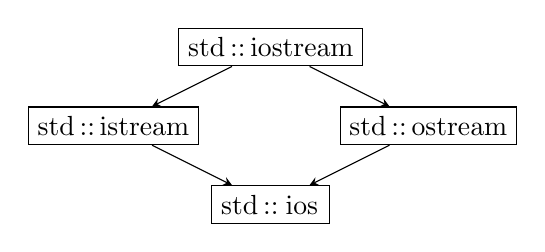
\begin{tikzpicture}
      \node[draw] (IO) at ( 0, 0) { \lstinline!std::iostream! } ;
      \node[draw] (I) at (-2,-1) { \lstinline!std::istream! } ;
      \node[draw] (O) at ( 2,-1) { \lstinline!std::ostream! } ;
      \node[draw] (B) at ( 0,-2) { \lstinline!std::ios! } ;

      \draw[->,>=stealth] (IO) -- (I) ;
      \draw[->,>=stealth] (IO) -- (O) ;
      \draw[->,>=stealth] (I) -- (B) ;
      \draw[->,>=stealth] (O) -- (B) ;
    \end{tikzpicture}
    \end{center}
  \end{example}
\end{frame}

\begin{frame}{Virtual base class}{}
  \begin{example}[Virtual base class]
    \sourceinput{snippets/virtual_base_class.cc}
  \end{example}
\end{frame}

% TODO: initialization of virtual base class?


\subsubsection{Empty Base Optimization (EBO)}

% Source: https://en.cppreference.com/w/cpp/language/ebo
\begin{frame}{Empty Base Optimization (EBO)}{}
  \begin{block}{Empty Base Optimization (EBO)}
    \strong{Empty Base Optimization} (EBO) allows the size of an empty base subobject to be zero
  \end{block}

  \begin{block}{Explanation}
    \begin{itemize}
    \item
      The size of any object or member subobject is required to be at least 1 even if the type is an empty class, in order to be able to guarantee that the addresses of distinct objects of the same type are always distinct.
    \item
      However, base class subobjects are not so constrained, and can be completely optimized out from the object layout
    \end{itemize}
  \end{block}
\end{frame}

\begin{frame}{Empty Base Optimization}{}
  \begin{example}[Empty Base Optimization]
    \sourceinput{snippets/ebo.cc}
  \end{example}
\end{frame}


\subsection{Polymorphism}

\subsubsection{Virtual functions}

% Source: https://en.cppreference.com/w/cpp/language/virtual
\begin{frame}{Virtual functions}{}
  \begin{definition}[Virtual function]
    A \strong{virtual function} is a non-static member function with the \lstinline!virtual! specifier. A virtual function supports dynamic dispatch, i.e. its behavior can be overridden in derived classes.
  \end{definition}

  \begin{block}{Virtual functions override}
    A function that overrides a virtual function in a derived class must have the same:
    \begin{itemize}
    \item
      name
    \item
      parameter type list (but not the return type)
    \item
      cv-qualifiers and ref qualifiers
    \end{itemize}
  \end{block}

  \begin{block}{Remark}
    A virtual function does not need to be visible (\lstinline!public! or \lstinline!protected!) to be overridden.
  \end{block}
\end{frame}

\begin{frame}{Virtual functions}{}
  \begin{example}[Virtual functions]
    \sourceinput{snippets/virtual_functions.cc}
  \end{example}
\end{frame}

% Source: https://en.cppreference.com/w/cpp/language/virtual
\begin{frame}{\texttt{override} and \texttt{final}}{}
  \begin{block}{\texttt{override} and \texttt{final}}
    \begin{itemize}
    \item
      If a function is declared with the specifier \lstinline!override!, but does not override a virtual function, the program is ill-formed
    \item
      If a function is declared with the specifier \lstinline!final!, and another function attempts to override it, the program is ill-formed
    \end{itemize}
  \end{block}
\end{frame}

\begin{frame}{\texttt{override} and \texttt{final}}{}
  \begin{example}[\texttt{override} and \texttt{final}]
    \sourceinput{snippets/override_and_final.cc}
  \end{example}
\end{frame}

\subsubsection{Virtual destructors}

% Source: https://en.cppreference.com/w/cpp/language/virtual
\begin{frame}{Virtual destructor}{}
  \begin{block}{Virtual destructor}
    Even though destructors are not inherited, if a base class declares its destructor virtual, the derived destructor always overrides it. This makes it possible to delete dynamically allocated objects of polymorphic type through pointers to base.
  \end{block}
  \begin{block}{Important remark}
    If a class is polymorphic (declares or inherits at least one virtual function), it must declare its destructor \lstinline!virtual!.
  \end{block}
\end{frame}

\begin{frame}{Virtual destructor}{}
  \begin{example}[Virtual destructor]
    \sourceinput{snippets/virtual_destructor.cc}
  \end{example}
\end{frame}

\subsubsection{Pure virtual functions}

% Source: https://en.cppreference.com/w/cpp/language/abstract_class
\begin{frame}{Pure virtual functions and abstract classes}{}
  \begin{definition}[Pure virtual function]
    A \strong{pure virtual function} is a virtual function with the \emph{pure specifier} noted \lstinline!= 0!.
  \end{definition}

  \begin{definition}[Abstract class]
    An \strong{abstract class} is a class that either defines or inherits at least one pure virtual function.
  \end{definition}

  \begin{block}{Remarks}
    \begin{itemize}
    \item
      No objects of an abstract class can be created
    \item
      Abstract classes are used as base classes for concrete classes
    \end{itemize}
  \end{block}
\end{frame}

\begin{frame}{Pure virtual functions and abstract classes}{}
  \begin{example}[Abstract class]
    \sourceinput{snippets/abstract_class.cc}
  \end{example}
\end{frame}

\subsubsection{Virtual table}

% Source: https://en.wikipedia.org/wiki/Virtual_method_table
\begin{frame}{Virtual table and virtual table pointer}{}
  \begin{definition}[Virtual table]
    A \strong{virtual table} (or vtable) is a per-class table containing function pointers to virtual functions. It is generated by the compiler.
  \end{definition}

  \begin{definition}[Virtual table pointer]
    A \strong{virtual table pointer} (or vptr) is a per-object pointer to a virtual table added by the constructor. The vptr is part of the object.
  \end{definition}

  \begin{block}{Call to a virtual function}
    \begin{enumerate}
    \item
      Fetch the virtual table pointer of the object
    \item
      Call the function declared in the table pointed by the virtual table pointer
    \end{enumerate}
    Consequence: calling a virtual function requires an indirection!
  \end{block}
\end{frame}

\begin{frame}{Virtual table and virtual table pointer}{}
  \begin{example}[Virtual table and virtual table pointer]
    \sourceinput{snippets/vtable_vptr.cc}
  \end{example}
\end{frame}

\subsubsection{Run-time type information (RTTI)}

% Source: https://en.cppreference.com/w/cpp/language/dynamic_cast
\begin{frame}{\texttt{dynamic\_cast}}{}
  \begin{block}{\texttt{dynamic\_cast}}
    A \strong{\lstinline!dynamic_cast!} safely converts pointers and references to classes up, down, and sideways along the inheritance hierarchy.

    {
      \hfill\lstinline[mathescape]!dynamic_cast<$type$>($expr$)!\hfill
    }

    \lstinline[mathescape]!$expr$! is:
    \begin{itemize}
    \item
      A glvalue of a complete class type if \lstinline[mathescape]!$type$! is a reference
    \item
      A prvalue of a pointer to a complete class type if \lstinline[mathescape]!$type$! is a pointer
    \end{itemize}
  \end{block}

  \begin{block}{Result of a \texttt{dynamic\_cast}}
    \begin{itemize}
    \item
      If the cast is successful, \lstinline!dynamic_cast! returns a value of type \lstinline[mathescape]!$type$!.
    \item
      If the cast fails and \lstinline[mathescape]!$type$! is a pointer type, it returns a null pointer.
    \item
      If the cast fails and \lstinline[mathescape]!$type$! is a reference type, it throws an exception that matches a handler of type \lstinline!std::bad_cast!.
    \end{itemize}
  \end{block}
\end{frame}

\begin{frame}{\texttt{dynamic\_cast}}{}
  \begin{example}[\texttt{dynamic\_cast}]
    \sourceinput{snippets/dynamic_cast.cc}
  \end{example}
\end{frame}

% Source: https://en.cppreference.com/w/cpp/language/typeid
\begin{frame}{\texttt{typeid}}{}
  \begin{block}{\texttt{typeid}}
    The \lstinline!typeid! operator queries information of a type and returns an object of type \lstinline!const std::type_info&!. It can be used:
    \begin{itemize}
    \item
      with a type
    \item
      with an expression
    \end{itemize}
  \end{block}

  \begin{block}{\texttt{typeid} with an expression}
    \begin{itemize}
    \item
      If the expression is a glvalue expression that identifies an object of a polymorphic type, the \lstinline!typeid! expression evaluates the expression and then refers to the \lstinline!std::type_info! object that represents the dynamic type of the expression
    \item
      If expression is not a glvalue expression of polymorphic type, \lstinline!typeid! does not evaluate the expression, and the \lstinline!std::type_info! object it identifies represents the static type of the expression
    \end{itemize}
  \end{block}
\end{frame}

\begin{frame}{\texttt{typeid}}{}
  \begin{example}[\texttt{typeid}]
    \sourceinput{snippets/typeid.cc}
  \end{example}
\end{frame}

\subsection{Idioms}

\subsubsection{PImpl My Ride}

% Source: https://en.cppreference.com/w/cpp/language/pimpl
% Source: https://cpppatterns.com/patterns/pimpl.html
% Source: https://wiki.qt.io/D-Pointer
\begin{frame}{PImpl: Pointer to Implementation}{}
  \begin{block}{PImpl: Pointer to Implementation}
    \strong{PImpl} (Pointer to Implementation) (a.k.a. d-pointer or opaque pointer) is a technique to hide implementation details of a class in order to achieve ABI stability.
  \end{block}

  \begin{block}{PImpl in practice}
    \sourceinput{snippets/pimpl.cc}
  \end{block}
\end{frame}

\begin{frame}{PImpl or not PImpl}{}
  \begin{block}{Advantages of PImpl}
    \begin{itemize}
    \item
      Compilation firewall: a modification in \lstinline!Impl! does not require a recompilation of all classes that use \lstinline!Foo!
    \item
      Move-friendly: a \lstinline!std::unique_ptr! is easy to move, especially in containers
    \end{itemize}
  \end{block}
  \begin{block}{Drawbacks of PImpl}
    \begin{itemize}
    \item
      Access overhead: an access to a member requires an indirection through a pointer
    \item
      Space overhead: the object requires an additional pointer
    \item
      Lifetime management: the implementation object is allocated on the heap
    \item
      Maintenance overhead: all the implementation has to be in a dedicated file
    \end{itemize}
  \end{block}
\end{frame}


\subsubsection{\texttt{const} correctness}

% Source: https://isocpp.org/wiki/faq/const-correctness
\begin{frame}{\texttt{const} correctness}{}
  \begin{block}{\texttt{const} correctness}
    \lstinline!const! correctness is a set of rules to offer a guarantee about the (non-)mutability of object:
    \begin{itemize}
    \item
      Choose reference to \lstinline!const! or pointer to \lstinline!const! for parameters if you do not intend to modify the parameters
    \item
      Make a member function \lstinline!const! if the function does not modify the object
    \item
      If a member function is \lstinline!const! and returns a reference to a member, the reference should be \lstinline!const! or the function should return by value
    \end{itemize}
  \end{block}

  \begin{block}{Benefits of \texttt{const} correctness}
    \begin{itemize}
    \item
      The caller has the guarantee that a variable or an object will not be modified
    \item
      The compiler ensures that the callee respects the contract by emitting an error in case of modification of a \lstinline!const! object
    \item
      The \lstinline!const! property is spread through member function calls
    \end{itemize}
  \end{block}
\end{frame}

% overload const/non-const
\begin{frame}{\texttt{const} correctness}{}
  \begin{example}[\texttt{const} correctness]
    \sourceinput{snippets/const_correctness.cc}
  \end{example}
\end{frame}



% (N)RVO

\part{Functional programming}

% algorithms
%
% functors
% lambda
%
% function pointer
%
% std::function
% std::bind
%
% member function pointer

\part{Generic programming}

\section{Generic programming}

\subsection{Type detection}

\begin{frame}{Automatic type detection}{}
  \begin{block}{Automatic type detection in \CC{11} and \CC{14}}
    \lstinline!auto! can be used to automatically detect a type in the following situations.
    \begin{itemize}
    \item
      Variable declaration: the type is determined from the initializer \\
      \lstinline!auto x = 1 + 2;! $\to$ \lstinline!int!
    \item
      Function declaration: the type is the trailing return type \\
      \lstinline!auto func(int x) -> int;! $\to$ \lstinline!int!
    \item
      Function declaration: the type is deduced from its return statement\Since{14} \\
      \lstinline!auto add(int x, double y) \{ return x + y; \}! $\to$ \lstinline!double!
    \item
      Variable declaration with \lstinline!decltype(auto)!: the type is deduced from the initializing expression using the rules for \lstinline!decltype!\Since{14}
    \item
      Function declaration with \lstinline!decltype(auto)!: the type is deduced from the return statement using the rules for \lstinline!decltype!\Since{14}
    \item
      Parameter declaration in a lambda expression (generic lambda)\Since{14} \\
      \lstinline![](auto x) \{ return x + 1; \}!
    \end{itemize}
  \end{block}
\end{frame}

\begin{frame}{Automatic type detection}{}
  \begin{block}{Automatic type detection in \CC{17} and \CC{20}}
    \lstinline!auto! can be used to automatically detect a type in the following situations.
    \begin{itemize}
    \item
      Template parameter: the type is deduced from the argument\Since{17} \\
      \lstinline!template<auto Param> class C \{ \};!
    \item
      Structure binding declaration\Since{17} \\
      \lstinline!auto [it, inserted] = dict.insert("Hello");!
    \item
      Function parameter declaration\Since{20} \\
      \lstinline!int sign(auto x) \{ return (x > 0) - (x < 0); \}!
    \end{itemize}
  \end{block}
\end{frame}

\begin{frame}{Type of an entity or expression}{}
  \begin{block}{Type of an entity}
    \lstinline!decltype! can be used to inspect the type of an entity:
    \begin{itemize}
    \item
      unparenthesized identifier
    \item
      unparenthesized class member access expression
    \end{itemize}
  \end{block}

  \begin{block}{Type of an expression}
    \lstinline!decltype! can be used to inspect the type of an expression of type \lstinline!T!:
    \begin{itemize}
    \item
      if the expression is an xvalue, then \lstinline!decltype! yields \lstinline!T&&!
    \item
      if the expression is an lvalue, then \lstinline!decltype! yields \lstinline!T&!
    \item
      if the expression is an prvalue, then \lstinline!decltype! yields \lstinline!T!
    \end{itemize}
  \end{block}

  \begin{block}{Warning!}
    For an identifier \lstinline!x!, \lstinline!decltype(x)! and \lstinline!decltype((x))! are often different types.
  \end{block}
\end{frame}

\begin{frame}{Type of an entity or expression}{}
  \begin{example}[Type of an entity or expression]
    \sourceinput{snippets/decltype.cc}
  \end{example}
\end{frame}

% https://herbsutter.com/2013/08/12/gotw-94-solution-aaa-style-almost-always-auto/

\begin{frame}{When to use automatic type detection?}{Two schools}
  \begin{block}{School \#1: Only when necessary and/or convenient}
    \begin{itemize}
    \item
      When the type has no name (e.g. lambda) \\
      \lstinline!auto f = [](int x) \{ return x + 1; \};!
    \item
      When the type is too long (e.g. iterator types) \\
      \lstinline!auto it = dict.find("Toto");!
    \item
      When the type name is redundant with its initializer \\
      \lstinline!auto ptr = std::make_unique<Foo>();!
    \end{itemize}
  \end{block}
  \begin{block}{School \#2: Almost Always Auto}
    Some people advocate for "Almost Always Auto" (AAA), even for simple types
    (e.g. \lstinline!auto i = std::size_t\{0\};! instead of \lstinline!std::size_t i = 0;!)
  \end{block}
  $\to$ Do as you want: be consistent, write readable and maintainable code
\end{frame}


% type traits
%
% SFINAE
%
% https://en.wikipedia.org/wiki/Curiously_recurring_template_pattern
%
% policy based programming

% https://en.cppreference.com/w/cpp/language/dependent_name

% if constexpr


% \part{Extras}

% Things that were in previous parts but were put here because the parts
% were already too long


\section{Introduction}

\subsection{Design Rules}

\begin{frame}{Design Rules (1/4)}{General rules}
  \begin{block}{General rules}
    \begin{enumerate}
    \item
      \CCLang's evolution must be driven by real problems.
    \item
      Don't get involved in a sterile quest for perfection.
    \item
      \CCLang must be useful \emph{now}.
    \item
      Every feature must have a reasonably obvious implementation.
    \item
      Always provide a transition path.
    \item
      \CCLang is a language, not a complete system.
    \item
      Provide comprehensive support for each supported style.
    \item
      Don't try to force people to use a specific programming style.
    \end{enumerate}
  \end{block}
\end{frame}

\begin{frame}{Design Rules (2/4)}{Design support rules}
  \begin{block}{Design support rules}
    \begin{enumerate}
    \item
      Support sound design notions.
    \item
      Provide facilities for program organization.
    \item
      Say what you mean.
    \item
      All features must be affordable.
    \item
      It is more important to allow a useful feature than to prevent every misuse.
    \item
      Support composition of software from separately developed parts.
    \end{enumerate}
  \end{block}
\end{frame}

\begin{frame}{Design Rules (3/4)}{Language-technical rules}
  \begin{block}{Language-technical rules}
    \begin{enumerate}
    \item
      No implicit violations of the static type system.
    \item
      Provide as good support for user-defined types as for built-in types.
    \item
      Locality is good.
    \item
      Avoid order dependencies.
    \item
      If in doubt, pick the variant of a feature that is easiest to teach.
    \item
      Syntax matters (often in perverse ways).
    \item
      Preprocessor usage should be eliminated.
    \end{enumerate}
  \end{block}
\end{frame}

\begin{frame}{Design Rules (4/4)}{Low-level programming support rules}
  \begin{block}{Low-level programming support rules}
    \begin{enumerate}
    \item
      Use traditional (dumb) linkers.
    \item
      No gratuitous incompatibilities with C.
    \item
      Leave no room for a lower-level language below C++ (except assembler).
    \item
      What you don’t use, you don’t pay for (zero-overhead rule).
    \item
      If in doubt, provide means for manual control.
    \end{enumerate}
  \end{block}
\end{frame}


\section*{The end}

\subsection*{That's all folks!}

\begin{frame}{That's all for now\ldots}{}
  \begin{block}{}
    \begin{center}
      Questions?
    \end{center}
  \end{block}
\end{frame}


% \begin{frame}{}{}
%   \begin{block}{}
%     \begin{itemize}
%     \item
%     \item
%     \end{itemize}
%   \end{block}
% \end{frame}

\end{document}
